\documentclass[xcolor=dvipsnames]{beamer}
\usepackage{xmpmulti}
\usepackage{comp2402}

% For source code:
\usepackage{minted}
\usepackage{mdframed}
\surroundwithmdframed{minted}

% For aligning tables
\usepackage{array}

\newcommand{\mi}[1]{\multiinclude[<+>][start=1,format=pdf]{#1}}

\title{Computer Architecture Through Binary Searching}
\author{Pat Morin}
\date{Carleton University}


\begin{document}

\begin{frame}
  \titlepage
  \centerline{
    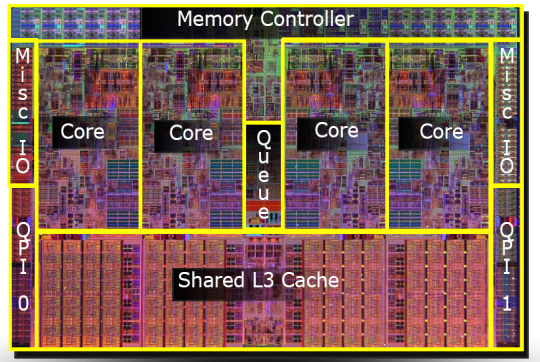
\includegraphics[height=1in]{images/nehalemdie}
    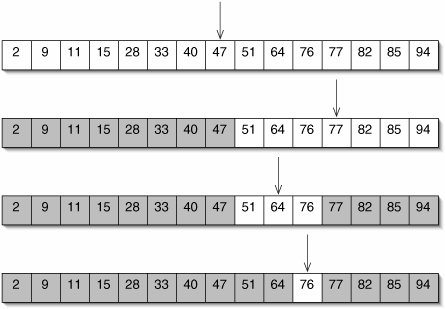
\includegraphics[height=1in]{images/binary-search}
    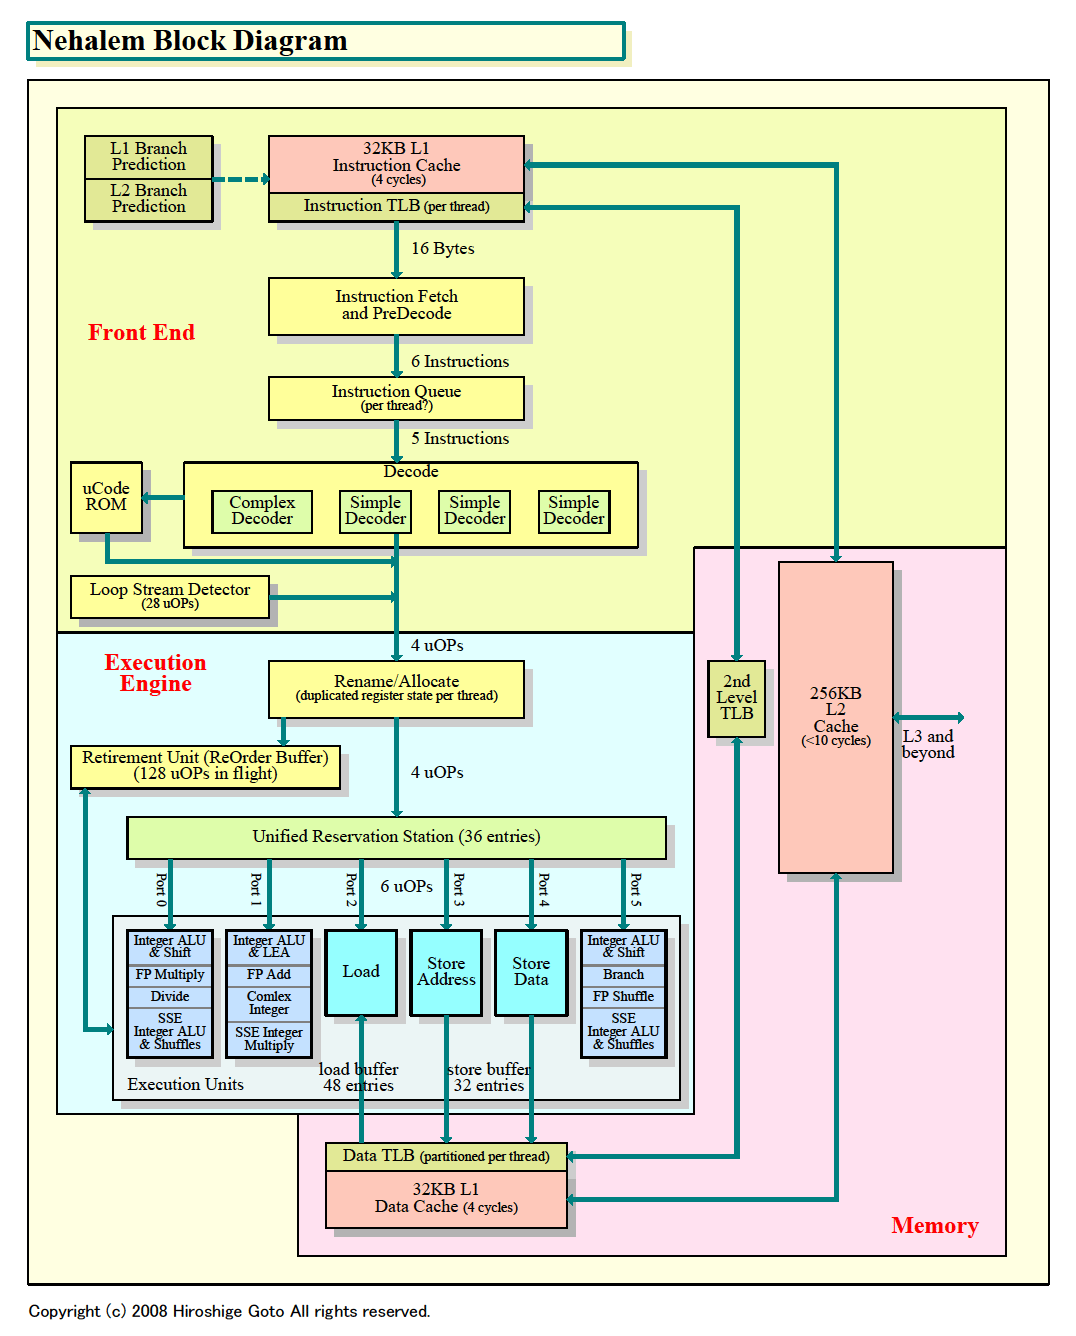
\includegraphics[height=1in]{images/nehalem-block}
  }
\end{frame}

\begin{frame}
  \frametitle{Microprocessor Architecture: Programmer's View}
  \framesubtitle{Von Neumann Architecture}

  \begin{center}
    \includegraphics[scale=0.85]{figs/programmers-view} 
  \end{center}
  
%  \begin{itemize}
%    \item<+->CPU repeatedly
%    \begin{itemize}
%      \item<+->Fetches an instruction (from RAM)
%      \item<+->Decodes the instruction
%      \item<+->Executes the instruction
%    \end{itemize}
%    \item<+->Instructions include:
%     \begin{itemize}
%      \item<+->Arithmetic operations on CPU registers
%      \item<+->Moving data between registers and RAM
%    \end{itemize}
%  \end{itemize}
  
\end{frame}


\begin{frame}
  \frametitle{Binary Search}
  \framesubtitle{The Classic Data Structure/Query Algorithm}

  \begin{center}
    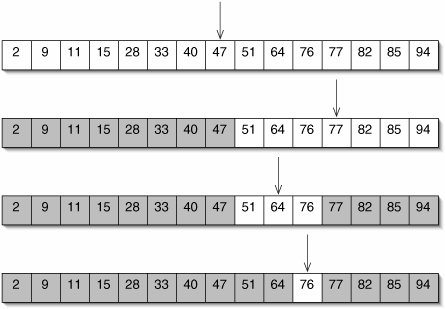
\includegraphics[width=.9\textwidth]{images/binary-search}
  \end{center}

\end{frame}


\begin{frame}[fragile]
  \frametitle{Binary Search}
  \framesubtitle{Branchy Code}

\begin{minted}{c++}
template<typename T, typename I>
I sorted_array<T,I>::branchy_search(T x) const {
    I lo = 0, hi = n;
    while (lo < hi) {
        I m = (lo + hi) / 2;
        if (x < a[m]) {
            hi = m;
        } else if (x > a[m]) {
            lo = m+1;
        } else {
            return m;
        }
    }
    return hi;
}
\end{minted}
\end{frame}

\begin{frame}[fragile]
  \frametitle{Binary Search: Analysis}

  \begin{itemize}
    \item<+->Each iteration of binary search either:
    \begin{itemize}
      \item<+->terminates (because \mintinline{c++}{x==a[m]})
      \item<+->terminates (because \mintinline{c++}{lo==hi})
      \item<+->Reduces \mintinline{c++}{hi-lo} by a factor of 2
    \end{itemize}
    \item<+->Binary search terminates after at most $\log_2 n$ iterations
    \item<+->Doubling the size of the array adds only one more iteration
  \end{itemize}
\end{frame}

\begin{frame}
  \frametitle{Binary Search: Experiments}
  \begin{center}
    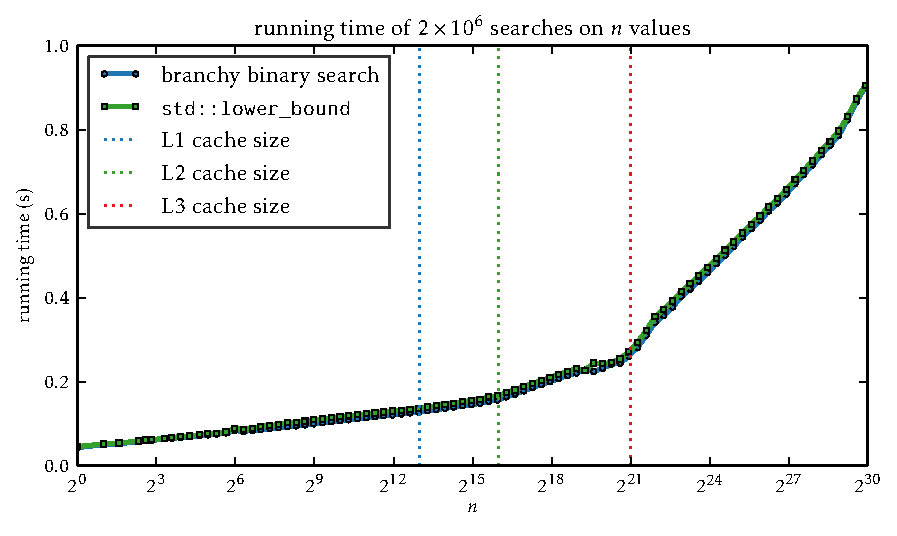
\includegraphics{graphs/sorted-i}
  \end{center}
\end{frame}

\begin{frame}[fragile]
  \frametitle{Binary Search}
  \framesubtitle{Branchy Assembly Code}

%\vspace{-2em}
\tiny
%\resizebox{\textwidth}{\textheight}{
\begin{minted}{nasm}
       .cfi_startproc
       movq    8(%rdi), %rax
       xorl    %ecx, %ecx
       movq    (%rdi), %r8
       cmpq    %rcx, %rax
       jbe     .L5                 ; quit if lo == hi
.L11:  leaq    (%rcx,%rax), %rdx   ; top of while loop
       shrq    %rdx
       movl    (%r8,%rdx,4), %edi  ; load a[m]
       cmpl    %edi, %esi          ; compare a[m] and x
       jnb    .L3                  ; jump if a[m] <= x
 .L8:  cmpq    %rdx, %rcx          ; a[m] > x, search first half
       movq    %rdx, %rax
       jnb     .L5
       addq    %rcx, %rdx          ; lo + hi
       shrq    %rdx                ; (lo + hi) / 2
       movl    (%r8,%rdx,4), %edi  ; load a[m]
       cmpl    %edi, %esi          ; compare a[m] and x
       jb      .L8                 ; jump if a[m] > x
 .L3:  cmpl    %edi, %esi          ; here a[m] <= x
       jbe     .L7                 ; quit if a[m] == x
       leaq    1(%rdx), %rcx
       cmpq    %rcx, %rax
       ja      .L11                ; back to top, if lo < hi
 .L5:  rep ret
 .L7:  movq    %rdx, %rax
       ret
       .cfi_endproc
\end{minted}
%}

\end{frame}

\begin{frame}
   \frametitle{The Instruction Pipeline}

   \begin{center}
      \mi{figs/pipeline}
   \end{center}
   \vspace{-1em}
   \begin{itemize}
     \item<3->Guess wrong and we have to flush the whole pipeline!
     \item<4->Nehalem architecture: pipeline is 20--24 cycles long
   \end{itemize}
\end{frame}

\begin{frame}[fragile]
   \frametitle{Branch-Free Binary Search}
   \framesubtitle{C++ Code}

   \begin{itemize}
       \item On random searches, branchy binary search will guess 
                wrong nearly 50\% of the time.
       \item Eliminate branching with conditional moves (\texttt{\color{blue}cmov})
   \end{itemize}
\begin{minted}{c++}
I sorted_array<T,I>::branchfree_search(T x) const {
  const T *base = a;
  I n = this->n;
  while (n > 1) {
    const I half = n / 2;
    base = (base[half] < x) ? &base[half] : base;
    n -= half;
  }
  return (*base < x) + base - a;
}
\end{minted}
\end{frame}

\begin{frame}[fragile]
   \frametitle{Branch-Free Binary Search}
   \framesubtitle{Assembly Code}

\tiny
\begin{minted}{nasm}
  .cfi_startproc
  movq    8(%rdi), %rdx       ; move n into rdx
  movq    (%rdi), %r8         ; move a into r8
  cmpq    $1, %rdx            ; compare n and 1
  movq    %r8, %rax           ; move base into rax
  jbe    .L2                  ; quit if n <= 1
.L3:
  movq    %rdx, %rcx          ; put n into rcx
  shrq    %rcx                ; rcx = half = n/2
  leaq    (%rax,%rcx,4), %rdi ; load &base[half] into rdi
  cmpl    %esi, (%rdi)        ; compare x and base[half]
  cmovb   %rdi, %rax          ; set base = &base[half] if x > base[half]
  subq    %rcx, %rdx          ; n = n - half
  cmpq    $1, %rdx            ; compare n and 1
  ja      .L3                   ; keep going if n > 1
.L2:
  cmpl    %esi, (%rax)        ; compare x to *base
  sbbq    %rdx, %rdx          ; set dx to 00..00 or 11...11
  andl    $4, %edx            ; set dx to 0 or 4 
  addq    %rdx, %rax          ; add dx to base
  subq    %r8, %rax           ; compute base - a (* 4)
  sarq    $2, %rax            ; (divide by 4)
  ret
  .cfi_endproc
\end{minted}
\end{frame}

\begin{frame}[fragile]
   \frametitle{Branch-Free Binary Search}
   \framesubtitle{Performance}

   \begin{center}
     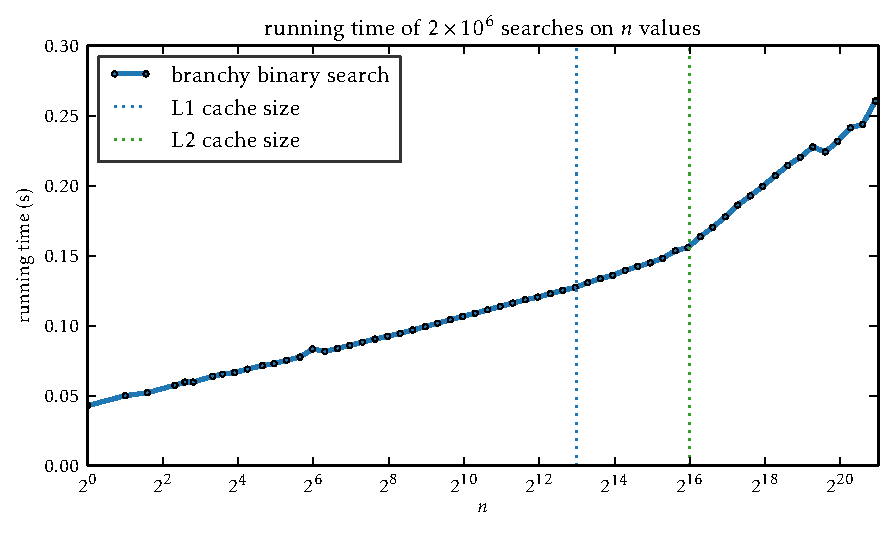
\includegraphics{graphs/sorted-ii}
   \end{center}
\end{frame}


\begin{frame}
   \frametitle{The Memory Hierarchy}

   \begin{center}
     \only<+>{\includegraphics[scale=0.85]{figs/programmers-view}}%
     \only<+->{\includegraphics[scale=0.85]{figs/caches}}
   \end{center}
   \begin{itemize}
     \item<+->Sizes: RAM (GB), L3 (MB), L2 (100's of KB), L1 (KB)
     \item<+->Speeds: RAM (100 cycles), L3 (40 cycles), L2 (10 cycles), L1 (4 cycles)
   \end{itemize}
   
\end{frame}

\begin{frame}
   \frametitle{Branch-Free Binary Search}
   \framesubtitle{Performance}

   \begin{center}
     \only<+>{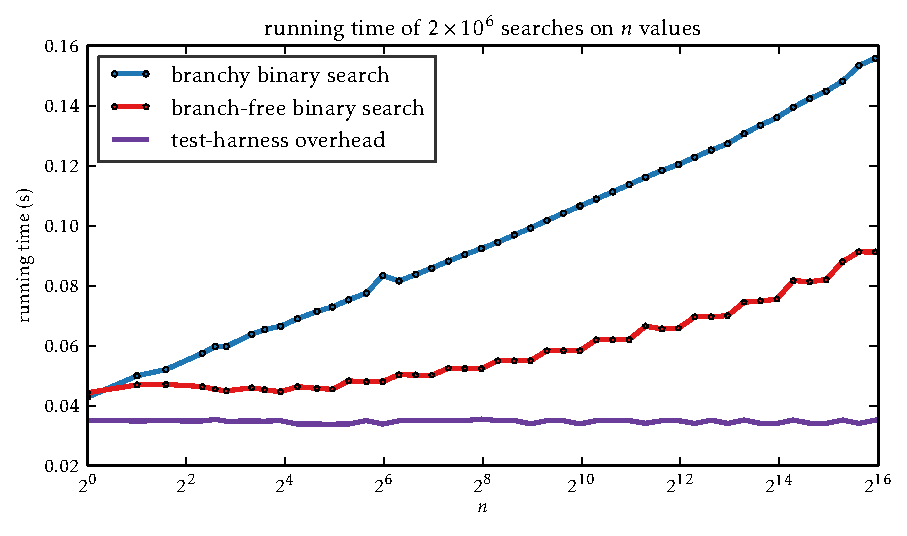
\includegraphics{graphs/sorted-iii}}%
     \only<+>{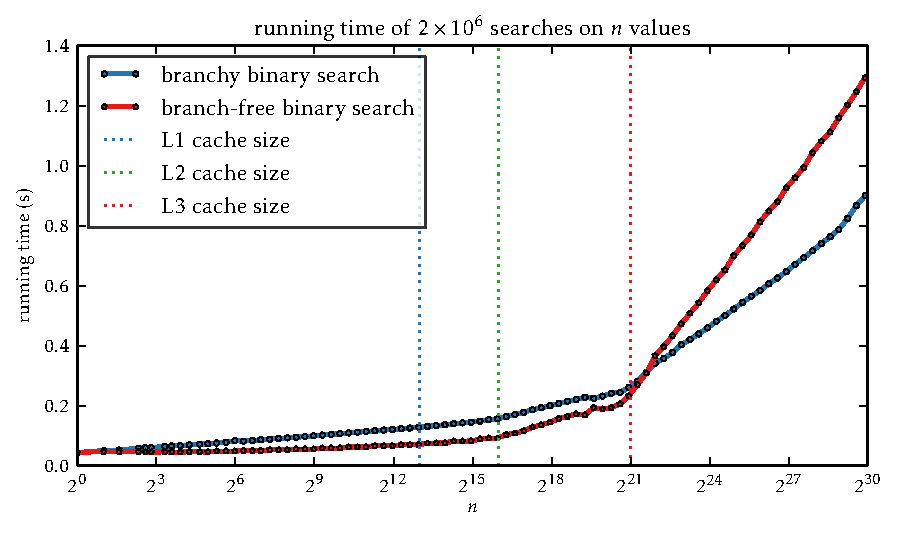
\includegraphics{graphs/sorted-iv}}%
     \only<+>{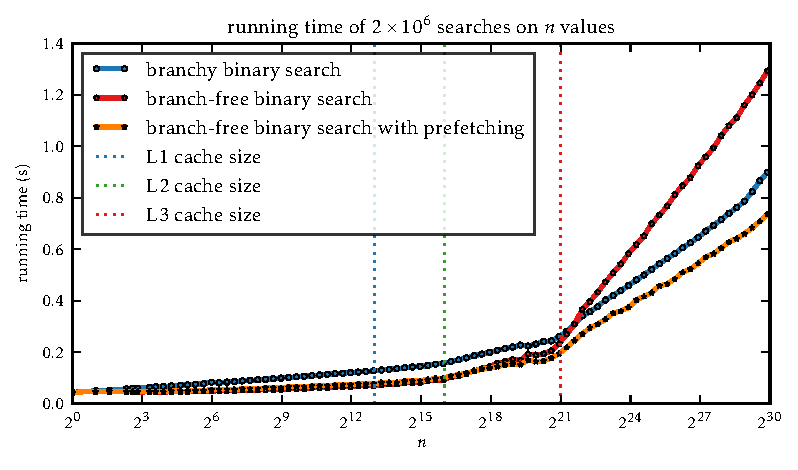
\includegraphics{graphs/sorted-v}}%
     \only<+->{\includegraphics[scale=0.85]{graphs/sorted-vi}\\[-2ex]{Wait, what?}}
   \end{center}
\end{frame}

\begin{frame}[fragile]
   \frametitle{Branchy versus Branch-Free Binary Search}
   \framesubtitle{Performance}

   \begin{tabular}{m{.48\textwidth}m{.48\textwidth}}
\tiny
 \begin{minted}{c++}
template<typename T, typename I>
I sorted_array<T,I>::branchy_search(T x) {
    I lo = 0, hi = n;
    while (lo < hi) {
        I m = (lo + hi) / 2;
        if (x < a[m]) {
            hi = m;
        } else if (x > a[m]) {
            lo = m+1;
        } else {
            return m;
        }
    }
    return hi;
}
\end{minted}
&
     \includegraphics[scale=0.5]{graphs/sorted-vi}
\end{tabular}
\begin{itemize}
  \item<+-> Branch-prediction is wrong $1/2$ the time
     \begin{itemize}
       \item<+-> Causes costly pipeline flush
     \end{itemize}
  \item<+-> Branch-prediction is right $1/2$ the time
      \begin{itemize}
       \item<+-> Puts memory subsystem to work loading from memory
     \end{itemize}
  \item<+->RAM latency $\approx100$ cycles, pipeline latency $\approx 20$ cycles
\end{itemize}
\end{frame}

\begin{frame}
   \frametitle{Cache Lines}

   \begin{itemize}
      \item<+-> RAM and caches are organized into \emph{lines}
      \begin{itemize}
        \item<+-> 64 bytes wide
      \end{itemize}
      \item<+-> Accessing a single word of RAM loads an entire line
         into the cache hierarchy
      \item<+-> Why?  Program is likely to access a nearby word soon,
         and it will already be in the cache
   \end{itemize}

\end{frame}

\end{document}

